\documentclass[a4paper]{article}

%% Language and font encodings
\usepackage[english]{babel}
\usepackage[utf8x]{inputenc}
\usepackage[T1]{fontenc}
\usepackage{listings}

%% Sets page size and margins
\usepackage[a4paper,top=3cm,bottom=2cm,left=3cm,right=3cm,marginparwidth=1.75cm]{geometry}

%% Useful packages
\usepackage{amsmath}
\usepackage[colorinlistoftodos]{todonotes}
\usepackage[colorlinks=true, allcolors=blue]{hyperref}
\usepackage{listings}
\usepackage{url}
\usepackage{graphicx}
\graphicspath{ {./images/} }
% \DeclareGraphicsExtensions{.pdf,.jpg,.png}

%% defined colors
\definecolor{Blue}{rgb}{0,0,0.5}
\definecolor{Green}{rgb}{0,0.75,0.0}
\definecolor{LightGray}{rgb}{0.6,0.6,0.6}
\definecolor{DarkGray}{rgb}{0.3,0.3,0.3}

% \newcommand*\lstinputpath[1]{\lstset{inputpath=#1}}
% \lstinputpath{code/}

\lstset{language=R,
   basicstyle=\ttfamily\small,
   breaklines=true,
   keywordstyle=\bfseries\color{Blue},
   commentstyle=\itshape\color{LightGray},
   stringstyle=\color{Green},
   numbers=left,
   numberstyle=\tiny\color{DarkGray},
   stepnumber=1,
   numbersep=10pt,
   backgroundcolor=\color{white},
   tabsize=2,
   showspaces=false,
   showstringspaces=false,
   captionpos=b,
%    inputpath={code/},
   frame=tb
}

\lstset{language=Python,
   basicstyle=\ttfamily\small,
   breaklines=true,
   keywordstyle=\bfseries\color{Blue},
   commentstyle=\itshape\color{LightGray},
   stringstyle=\color{Green},
   numbers=left,
   numberstyle=\tiny\color{DarkGray},
   stepnumber=1,
   numbersep=10pt,
   backgroundcolor=\color{white},
   tabsize=2,
   showspaces=false,
   showstringspaces=false,
   captionpos=b,
%    inputpath={code/},
   frame=tb
}

\lstset{language=Matlab,
   basicstyle=\ttfamily\small,
   breaklines=true,
   keywordstyle=\bfseries\color{Blue},
   commentstyle=\itshape\color{LightGray},
   stringstyle=\color{Green},
   numbers=left,
   numberstyle=\tiny\color{DarkGray},
   stepnumber=1,
   numbersep=10pt,
   backgroundcolor=\color{white},
   tabsize=2,
   showspaces=false,
   showstringspaces=false,
   captionpos=b,
%    inputpath={code/},
   frame=tb
}

\title{IDS 2017 \\Assignment 1}
\author{
 Bogdan Petre (s3480941) \\ 
 Low Daniel (s3120155) \\
 Xu Teng Andrea (s3548120) 
 \\ \textbf{Group} 7}
\date{\today}


\begin{document}
\maketitle
\section{}
\subsection{Identify Data Types (10P)}

	\begin{itemize}
		\item Brightness as measured by a light meter: continuous because each measurement obtains a distinct score[1], quantitative (ratio) because this device could have an absolute zero (i.e., absence of light). 
		
		\item Brightness as measured by people’s judgments: if you use a Lickert scale to measure people’s judgment, then brightness would be discrete and qualitative (ordinal) becuase the measurements have a logical order but do not reflect numerical true values.  
		
		\item Time in terms of AM or PM: binary, qualitative (nominal if one considers there is not a logical order between AM and PM or ordinal if one views PM coming after AM).
		
		\item Coat check number (certain places offer you to leave your coat to someone who, in turn, gives
		you a number tag that you need to claim it back when you leave): discrete, qualitative (ordinal or perhaps nominal if the coats aren’t placed in the order of the integers).
	\end{itemize}

	\subsection{Collect It... Link it! (50P)}
	
	In this exercise we created enrich\_script.R in order to collect additional data from the API of OMDB. A general description of the code is provided in the \textit{ReadMe.txt} file, while more detailed explanations are given as comments.
	
	\subsection{Think About Types (20P)}
	
	\begin{itemize}
		\item Title: discrete, qualitative (nominal)
		Discrete because there is a finite number of titles and qualitative nominal because it's like an ID
		
		\item ReleaseDate: discrete, quantitative (interval)
		
		Discrete for the same reason, and quantitative (interval) because they are calendar dates.
		
		\item Popularity: continuous, quantitative (ratio)
		
		It's continuos because there infinite numbers of popularity since they are real numbers and quantitative (ratio) because there is absolute zero
		
		\item Budget: continuous, quantitative (ratio)
		
		same reason as above
		
		\item Revenue: continuous, quantitative (ratio)
		
		same reason as above
		
		\item Genre: discrete, categorical (nominal)
		
		discrete because there are finite number of genres, qualitative (nominal) you cannot declare an order
		
		\item imdbRating: discrete, numeric (ratio)
		
		discrete because it has a precision to the first decimal number , it exists the absolute zero
		
		\item imdbVotes: continuos, quantitative (ratio)
		
		it's continuos because there is no finite number of imdbVotes, and ratio because we can have 0 votes.
		 
		\item Director: discrete, categorical(nominal)
		
		discrete because there finite number of names, categorical (nominal) because they are names 
		 
		\item Country: discrete, qualitative (categorical)
			
		 same reason as above
		 
		\item PG rating: discrete, qualitative (ordinal)
		
		finite number of pg ratings, qualitative (ordinal ) because you can order the ratings by the age the child can watch that movie
		
	\end{itemize}

	\subsection{And Finally... Analyze it! 20P}
	
	\subsubsection{a}
	
	\begin{itemize}
		\item \textbf{Figure 1} Popularity follows a power law distribution with most movies having a popularity of 0 and 0.5.
		\begin{figure}[h]
		\begin{center}
		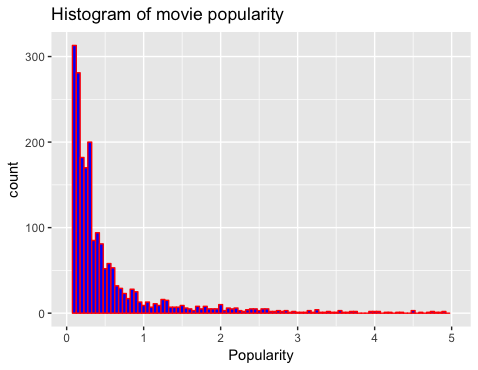
\includegraphics[width=0.8\textwidth]{fig_1_histogram_popularity}
		\caption{Histogram of popularity}
		\label{fig:f1}
		\end{center}
		\end{figure}
		\item \textbf{Figure 2} Continuous variables like popularity are better visualized with a density plot.
		\begin{figure}[h]
		\begin{center}
		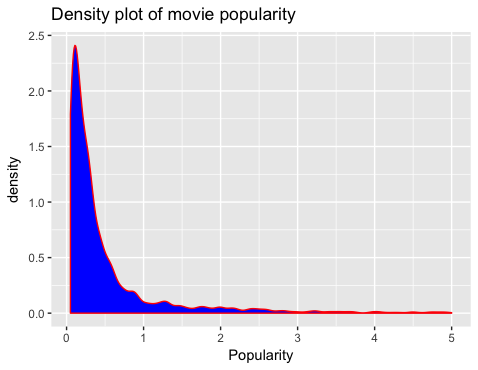
\includegraphics[width=0.8\textwidth]{fig_2_density_popularity}
		\caption{Density plot of popularity.}
		\label{fig:f2}
		\end{center}
		\end{figure}
		\item \textbf{Figure 3} Budget follows a power law distribution with most movies having spent less than 25 million dollars.
		\begin{figure}[h]
		\begin{center}
		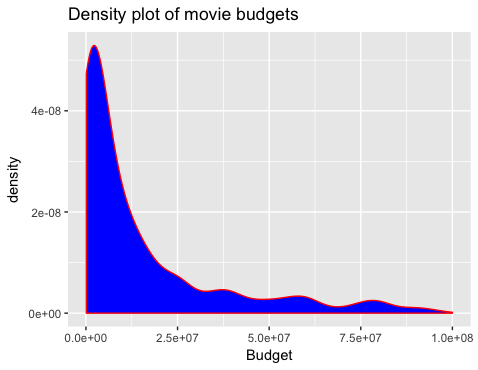
\includegraphics[width=0.8\textwidth]{fig_3_density_budget}
		\caption{Density plot of budget.}
		\label{fig:f3}
		\end{center}
		\end{figure}
		\item \textbf{Figure 4}
		Boxplot of most frequent genres shows that Comedy is the most frequent genre.
		\begin{figure}[h]
		\begin{center}
		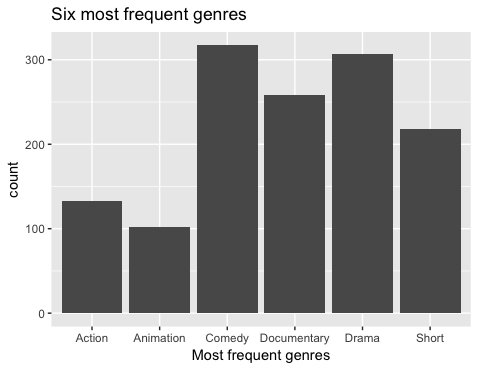
\includegraphics[width=0.8\textwidth]{fig_4_boxplot_genres}
		\caption{Most frequent genres}
		\label{fig:f4}
		\end{center}
		\end{figure}
	\end{itemize}
	
	
	
	\subsubsection{b}
	
	\begin{itemize}
		\item \textbf{Figure 5}\\
		\textbf{Does a higher budget produce a higher rating movie?}
		Interestingly, there seems to be a negative correlation with the movies spending more having a lower rating. But inferential statistics are needed to determine this. Moreover, very few movies had budgets reported, so more data is needed. 
		\begin{figure}[h]
		\begin{center}
		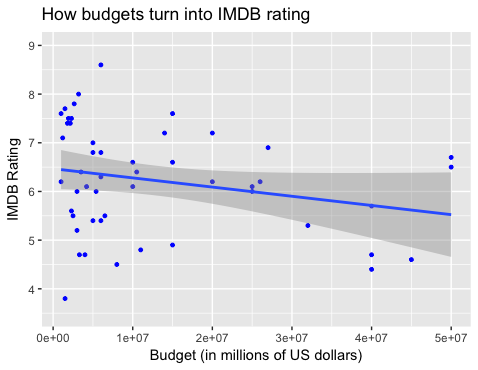
\includegraphics[width=0.8\textwidth]{fig_5_scatterplot_budget_rating}
		\caption{Scatter plot of budget and IMDB rating}
		\label{fig:f5}
		\end{center}
		\end{figure}   
		
		
		\item \textbf{Figure 6}\\
		 \textbf{Does a higher budget produce a more popular movie?}
		 Popularity weighs the rating on the amount of votes, so it can be considered as a better measure of general audience appeal than IMDB rating. There does not seem to be a trend; however, over 10 million dollars in budget, there seems to be a slight positive correlation (i.e., producing higher popularity). But inferential statistics are needed to determine this. Moreover, very few movies had budgets reported, so more data is needed.
		\begin{figure}[h]
		\begin{center}
		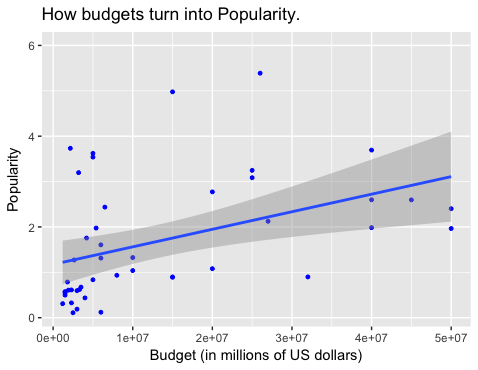
\includegraphics[width=0.8\textwidth]{fig_6_budget_popularity}
		\caption{Scatter plot of budget and popularity}
		\label{fig:f6}
		\end{center}
		\end{figure}      
		
		
		\item \textbf{Figure 7} 
		\textbf{Are certain genres more popular than others?}
		Popularity of most frequent genres shows a power law distribution. Short films have a bimodal distribution, with a most of the short films having a low score but also certain short films having a high rating over 5. It is difficult to answer this question with this figure alone, but for instance we can conclude that action movies seem to have higher popularity than others.
		\begin{figure}[h]
		\begin{center}
		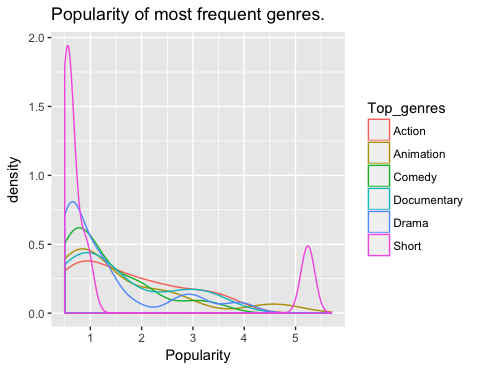
\includegraphics[width=0.8\textwidth]{fig_7_popularity_top_genres}
		\caption{Popularity of most frequent genres}
		\label{fig:f7}
		\end{center}
		\end{figure}   
	\end{itemize}
		
	\subsection{Bonus (+10P)}
	
	\textbf{1}\\
	We used a scatter plot in order to visualize the data that we have and compare properly the IMDB ratings and Rotten Tomatoes ratings. We can easily see that for some movie the ratings are pretty close for other there is some difference.
	That's because IMDB uses a weigthed mean [2] with all the users votes, in the other hand Rotten Tomatoes collects all the ratings from critical professionist from all over the world. There is also a Rotten Tomatoes rating from the users see [3].
		\begin{figure}[h]
		\begin{center}
		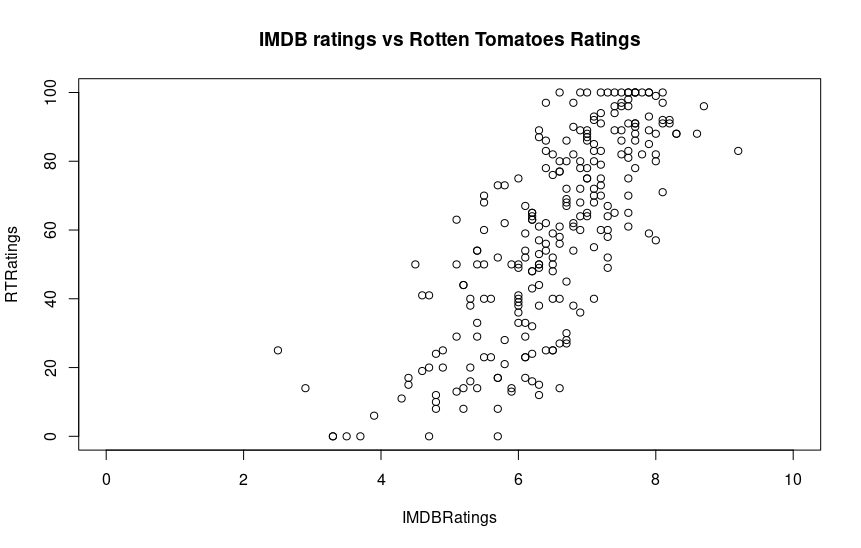
\includegraphics[width=0.8\textwidth]{imdb_vs_rottenR}
		\caption{IMDB vs. Rotten Tomatoes ratings}
		\label{fig:f8}
		\end{center}
		\end{figure}  

	\textbf{3}\\
	For this exercise we obtained also the Production House Information, then obtained the first Genre for every Movie in Order to delete noise with the other subGenres.\\
	Furthermore we obtained top10 Production Houses and then grouped each Production House with their genres counting per genre.\\
	So with a simple group by function we can easily see in the groupedGenrePerProduction.csv that usually each production house is used to one genre and maybe one or two outliers.

% citation section
\newpage
\begin{thebibliography}{9}
	\bibitem{DiscoveringStatistics}
	Field, A. (2009). Discovering statistics using SPSS. Sage publications. 
	
	\bibitem{IMDB rating}
	https://math.stackexchange.com/questions/169032/understanding-the-imdb-weighted-rating-function-for-usage-on-my-own-website
	
	\bibitem{Rotten rating}
	https://www.rottentomatoes.com/about/
\end{thebibliography}


\end{document}